\documentclass[conference]{IEEEtran}
\usepackage[pdftex]{graphicx}
\usepackage{hyperref}
\usepackage{float}
\graphicspath{{images/}}
\DeclareGraphicsExtensions{.pdf,.jpeg,.png}

\begin{document}
\hyphenation{op-tical net-works semi-conduc-tor}

\urlstyle{tt}

\title{CarSensor: Smart Street-side Parking with the Internet of Things}

\author{\IEEEauthorblockN{Daniel Lynch}
	\IEEEauthorblockA{Deparment of Mechanical Engineering\\
		Northwestern University\\
		2145 Sheridan Road\\
		Evanston, IL 60208, USA\\
		\texttt{daniellynch2021@u.northwestern.edu}}
	\and
	\IEEEauthorblockN{Yong Zhao}
	\IEEEauthorblockA{MPM Program\\
		Northwestern University\\
		2145 Sheridan Road\\
		Evanston, IL 60208, USA\\
		\texttt{yongzhao2019@u.northwestern.edu}}
	}
	
\maketitle

\begin{abstract}
We propose \texttt{CarSensor}, a networked array of sensors that provides parking information to users via a smartphone app. The design is guided by a desire for simplicity and modularity, two important attributes of Internet-of-Things systems and of cyberphysical systems in general. We describe our proof-of-concept prototype, built using popular open-source hardware and software. Based on this prototype, we then identify areas for further development that constitute prerequisites for full-scale implementation.
\end{abstract}

\section{Introduction}\label{sec_intro}
The recent surge in popularity of the Internet of Things (IoT) highlights some fundamental aspects of the design and analysis of cyberphysical systems, such as deterministic behavior, robustness, and extensibility. For the final project of EECS 395/495 Cyberphysical Systems (Winter 2018), we created \texttt{CarSensor} \footnote{\url{https://github.com/yongllyong123/project-1}}, a prototype of an IoT-inspired system for smarter street-side parking, which addressed these aforementioned aspects of cyberphysical systems. The remainder of this paper is structured as follows: Section~\ref{sec_intro} presents the motivation for this project, outlines the system-level design, and demonstrates where the system would be used. Section~\ref{sec_phys} details the physical components of the system and their low-level intercommunications. Section~\ref{sec_network} details the networked structure of the system and the high-level communication between components. Section~\ref{sec_futurework} presents some insights we gained while working on the project. Lastly, Section~\ref{sec_conc} concludes this report.

\subsection{Motivation}
Street parking can be a hassle, especially in urban areas. Knowing which parking spaces are full or empty can save a lot of time and aggravation. One way to realize this is by outfitting a street with an IoT system consisting of networked sensors and a client application all communicating with a central hub.

\subsection{Modular System Design}
\texttt{CarSensor} is intended to be modular, so that it can be expanded to support an arbitrary number of parking spaces. As shown in Figure~\ref{fig_blockdiagram}, \texttt{CarSensor} consists of three components:
\begin{itemize}
\item an arbitrary number of \textit{sensor modules} located at parking spaces,
\item a \textit{server} that collects data from the sensor modules and reasons about the state of each parking space, and
\item a \textit{smartphone app} that provides parking information to the end user.
\end{itemize}

\begin{figure}[h]
\centering
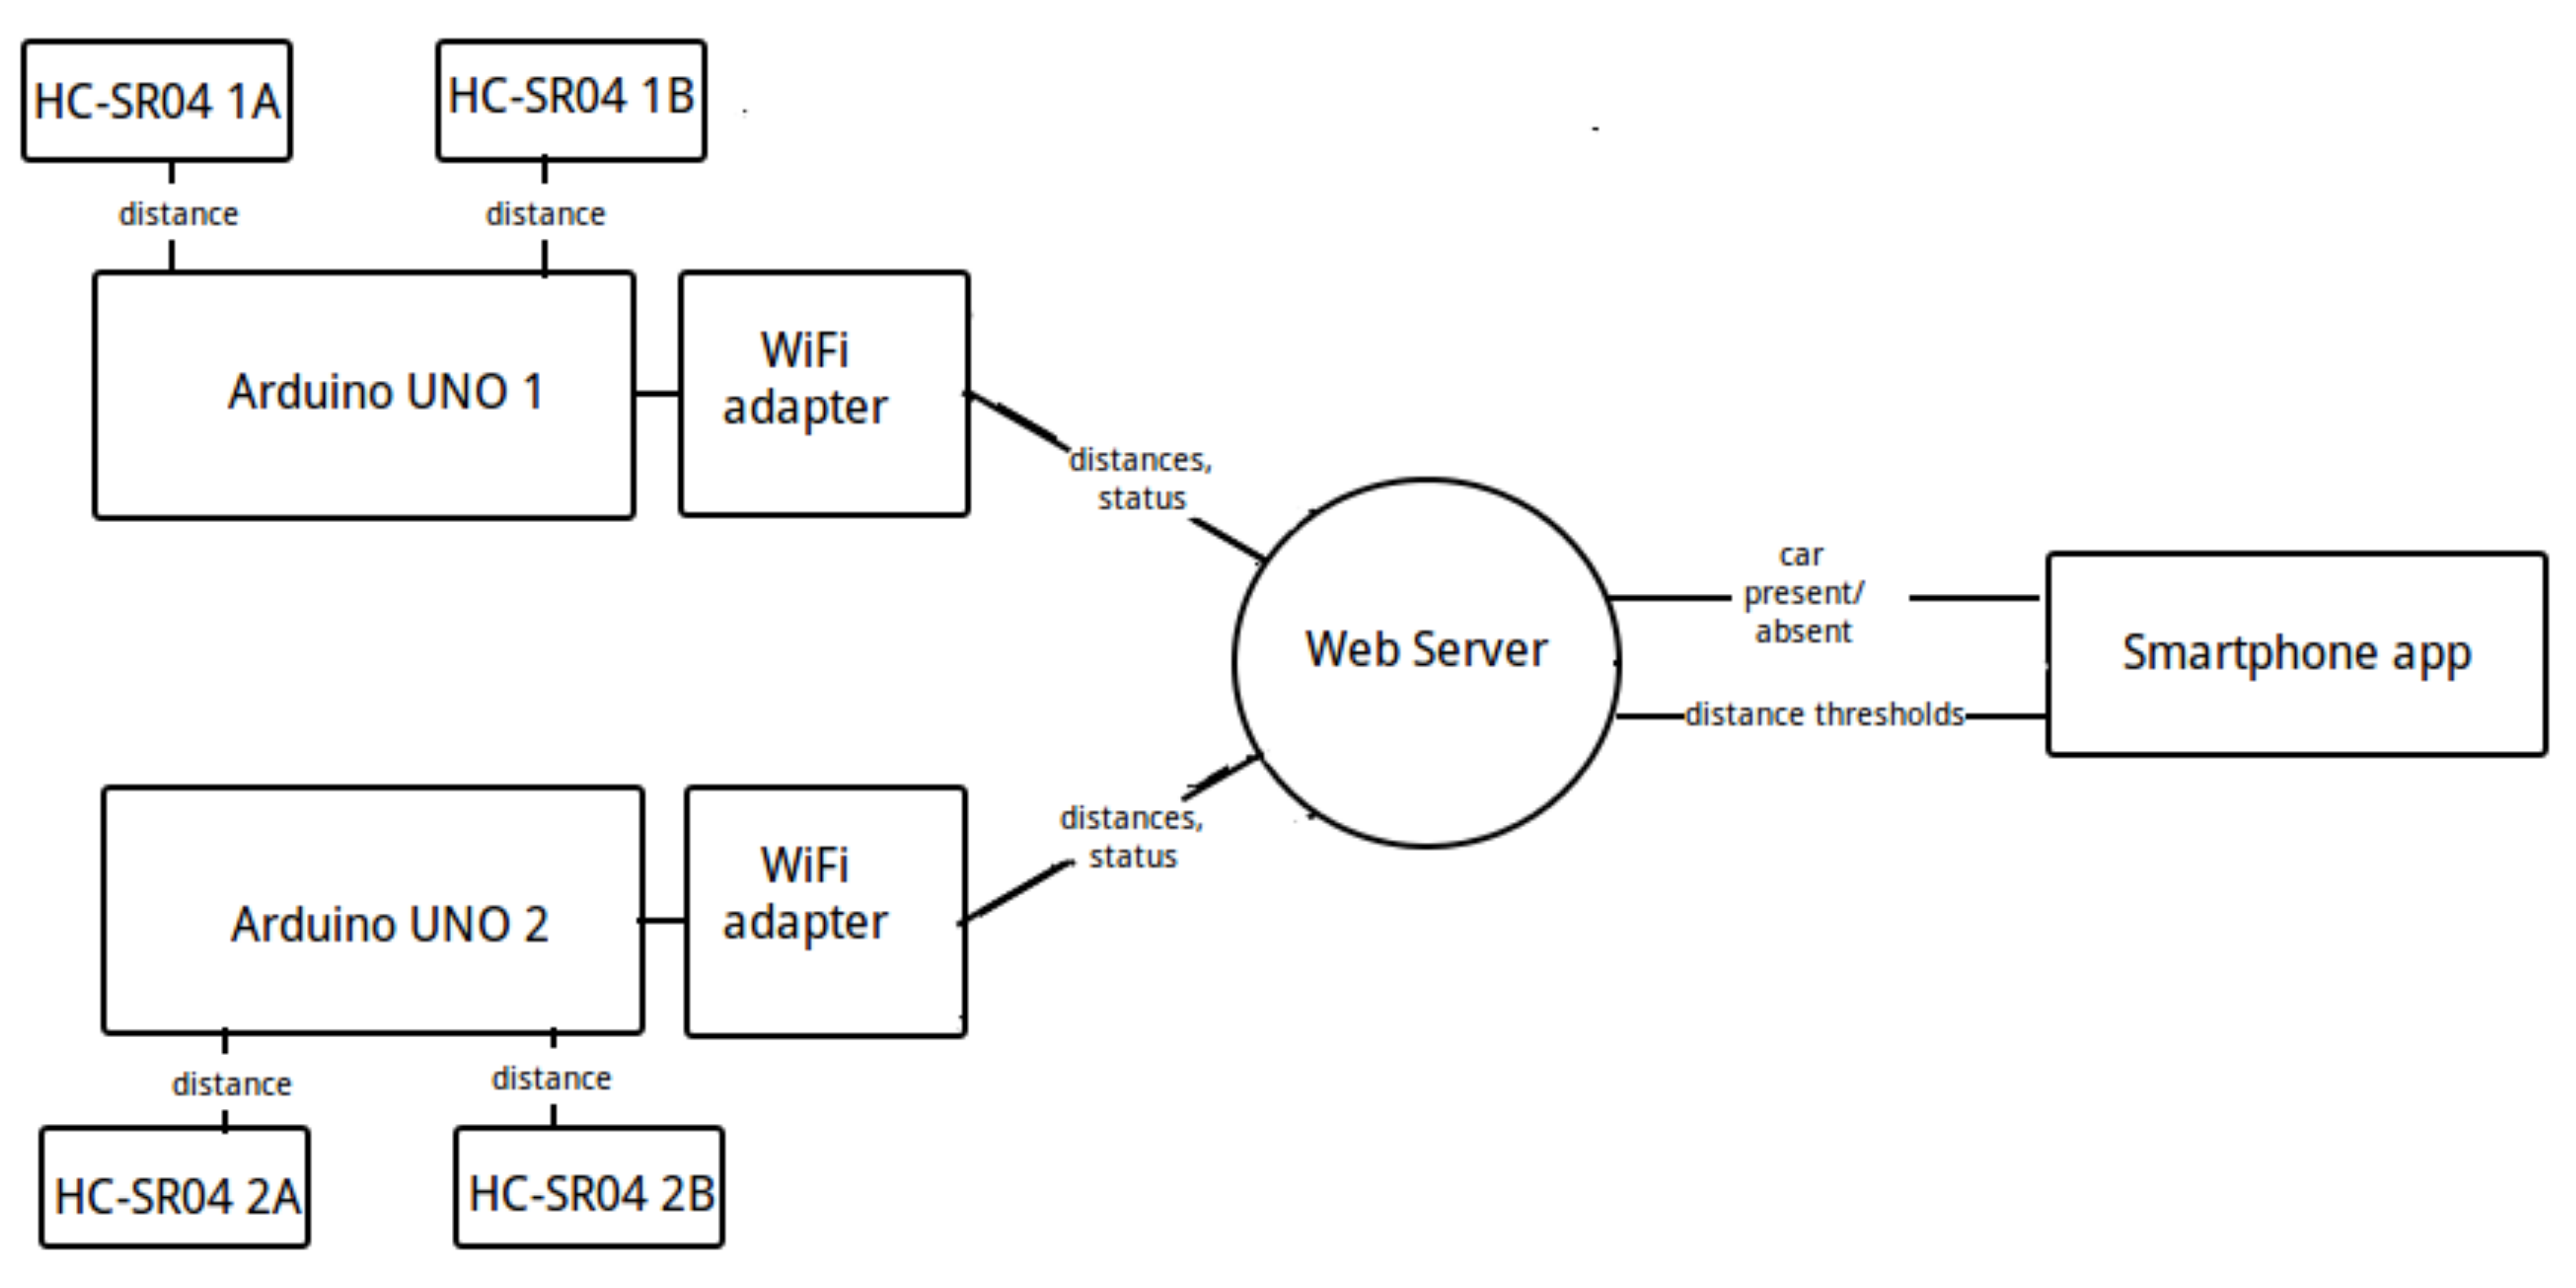
\includegraphics[width=3.0in]{block_diagram_0.png}
\caption{Block diagram of components used in our \texttt{CarSensor} prototype.}
\label{fig_blockdiagram}
\end{figure}

Each sensor module consists of two sensors, a microcontroller, and a network adapter. Each module is responsible for sensing two adjacent parking spaces, as shown in Figure~\ref{fig_curb}. The parking space in the middle of the figure is sensed by module 1's sensor B and module 2's sensor A; the parking space on the right would be sensed by module 2's sensor B and module 3's sensor A, and so on.
\begin{figure}[h]
\centering
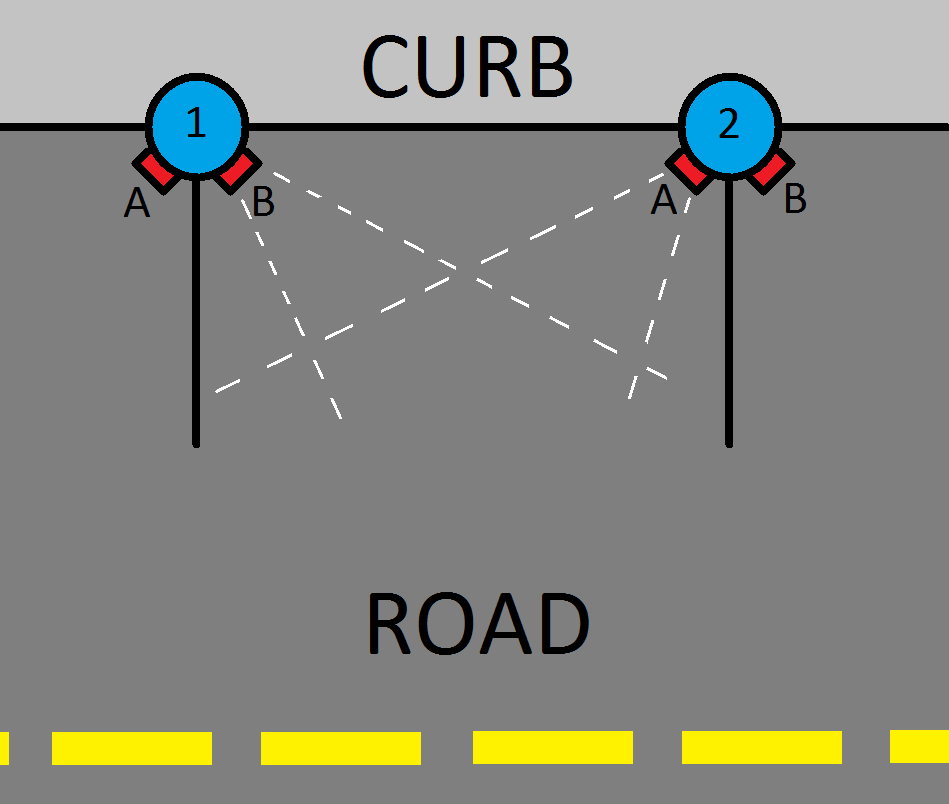
\includegraphics[width=2.0in]{parkingspace.png}
\caption{Physical layout of networked sensors used in \texttt{CarSensor}.}
\label{fig_curb}
\end{figure}

Each sensor module must also have a unique network identifier related to its physical location to allow the server to reason about the state of each parking space. In our prototype, we used IP addresses, but the limitations of that approach will be discussed in Section~\ref{sec_futurework}.

\section{Physical Layer}\label{sec_phys}
Our prototype design was motivated by the desire for fast and efficient development: we selected components that were easy to get up and running, bearing in mind that we were only developing a prototype rather than a production-ready system.

\subsection{Arduino UNO microcontroller}

\begin{figure}[h]
	\centering
	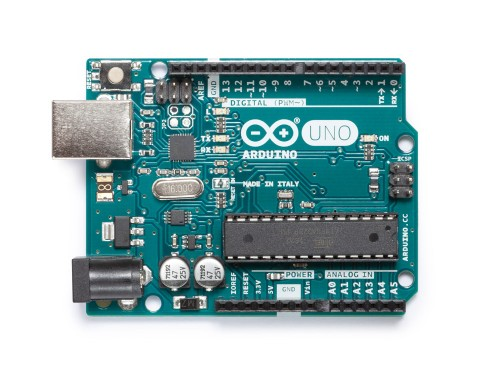
\includegraphics[width=2.5in]{arduinoUNO.jpg}
	\caption{Arduino UNO (image credit: Arduino)}
	\label{fig_arduinoUNO}
\end{figure}

Shown in Figure~\ref{fig_arduinoUNO}, the Arduino UNO is an open-source development board built around the ATmega328P microcontroller and has become a popular platform for prototyping simple embedded applications. We selected it for its overall ease of use, due to its integrated development environment (IDE) and the large user base.

\subsection{HC-SR04 ultrasonic distance sensor}

\begin{figure}[h]
	\centering
	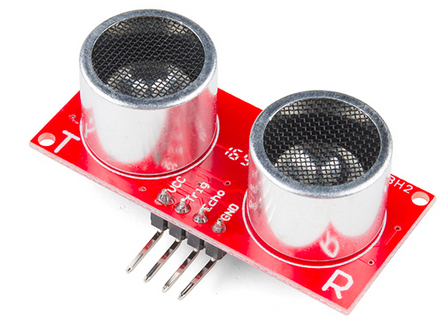
\includegraphics[width=2.0in]{hcsr04.png}
	\caption{HC-SR04 ultrasonic distance sensor (image credit: SparkFun Electronics \textsuperscript{\textregistered})}
	\label{fig_hcsr04}
\end{figure}

The HC-SR04 sensor, pictured in Figure~\ref{fig_hcsr04}, has two communication pins: \texttt{TRIG} (a digital input) and \texttt{ECHO} (a digital output). Its operational principle is similar to sonar: when \texttt{TRIG} is toggled high, the sensor emits an ultrasonic pulse; if an object reflects the pulse back to the sensor, it sets \texttt{ECHO} high. The microcontroller simply times the delay between setting \texttt{TRIG} high and receiving a logical 1 on \texttt{ECHO} and multiplies that time by the speed of sound (343 m/s in air at sea level) to estimate how far away the object is.

\texttt{CarSensor} is more concerned with detecting the presence of a vehicle in a parking space than with measuring distance, so measurements made with the HC-SR04 are compared to a heuristic distance threshold. If the measured distance is less than the threshold, a \texttt{proximity} bit, specific to that sensor, is set to 1 and subsequently sent to the server via the WiFi adapter; otherwise, \texttt{proximity} is set to 0 and then sent to the server. Since each Arduino uses two HC-SR04 sensors, each Arduino sends two \texttt{proximity} bits to the server, delimited by a space. This transmission occurs at a regular frequency (0.5 Hz in our prototype) and will be expanded on in Section~\ref{sec_futurework}.

\subsection{ESP8266 WiFi adapter}

\begin{figure}[h]
	\centering
	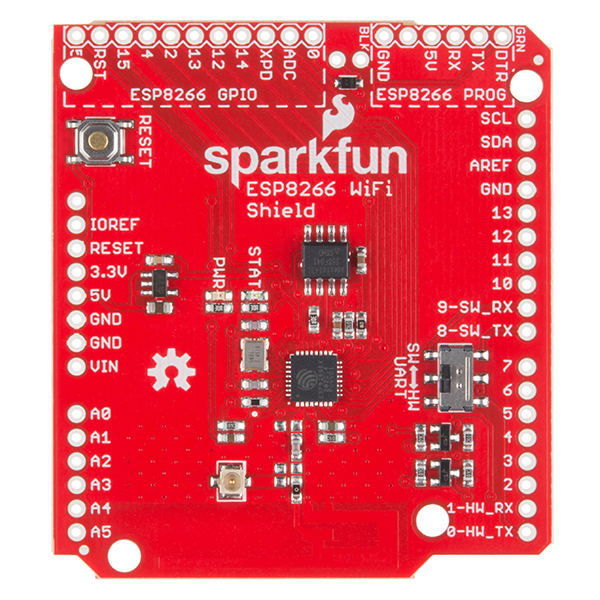
\includegraphics[width=2.0in]{esp8266.jpg}
	\caption{SparkFun ESP8266 WiFi shield for Arduino UNO (image credit: SparkFun Electronics \textsuperscript{\textregistered})}
	\label{fig_esp8266}
\end{figure}

After selecting our microcontroller, we needed to select a compatible WiFi adapter. We chose SparkFun's ESP8266 shield, pictured in Figure~\ref{fig_esp8266}, which is built around the ESP8266 system-on-a-chip (SoC) and provides TCP server and client functionality. It interfaces with the Arduino UNO over ``software serial,'' leaving the Arduino UNO's hardware serial port available for other communication uses (debugging via a terminal emulator, in our case). We used SparkFun's Arduino library and starter code\footnote{\url{https://github.com/sparkfun/SparkFun_ESP8266_AT_Arduino_Library}} to shorten the learning curve associated with using the ESP8266.

\section{Network Layer}\label{sec_network}
\subsection{Sensor clients}
Using the ESP8266 in TCP client mode, each Arduino UNO sends proximity information from both HC-SR04 sensors to the server at 0.5 Hz.
\subsection{Server}
We used \texttt{Node.js}\textsuperscript{\textregistered} \footnote{\url{https://nodejs.org/en/}} to develop a rudimentary server to collect data from each sensor module and handle requests from the smartphone app. Specifically, we used the \texttt{net}\footnote{\url{https://nodejs.org/api/net.html\#net_net}} module to create an asynchronous streaming TCP server that listens for requests on two ports (one for sensor modules, another for the smartphone app). In our prototype, we ran the server on a Lenovo laptop running Ubuntu 14.04 LTS.
\subsubsection{TCP sockets}
Sensor modules communicate with the server on port 8080, and the smartphone app communicates with the server on port 8000. This decision was motivated by the need for a modular system. Moreover, it simplifies the server design because TCP requests from the smartphone app do not need to be filtered out from sensor modules' TCP requests.
\subsubsection{State machine}
The core of \texttt{CarSensor} is a simple finite state machine (FSM) running on the server. As shown in Figure~\ref{fig_fsm}, the FSM has four states:
\begin{itemize}
\item \texttt{empty},
\item \texttt{pending full},
\item \texttt{full}, and
\item \texttt{pending empty}.
\end{itemize}
\begin{figure}[h]
	\centering
	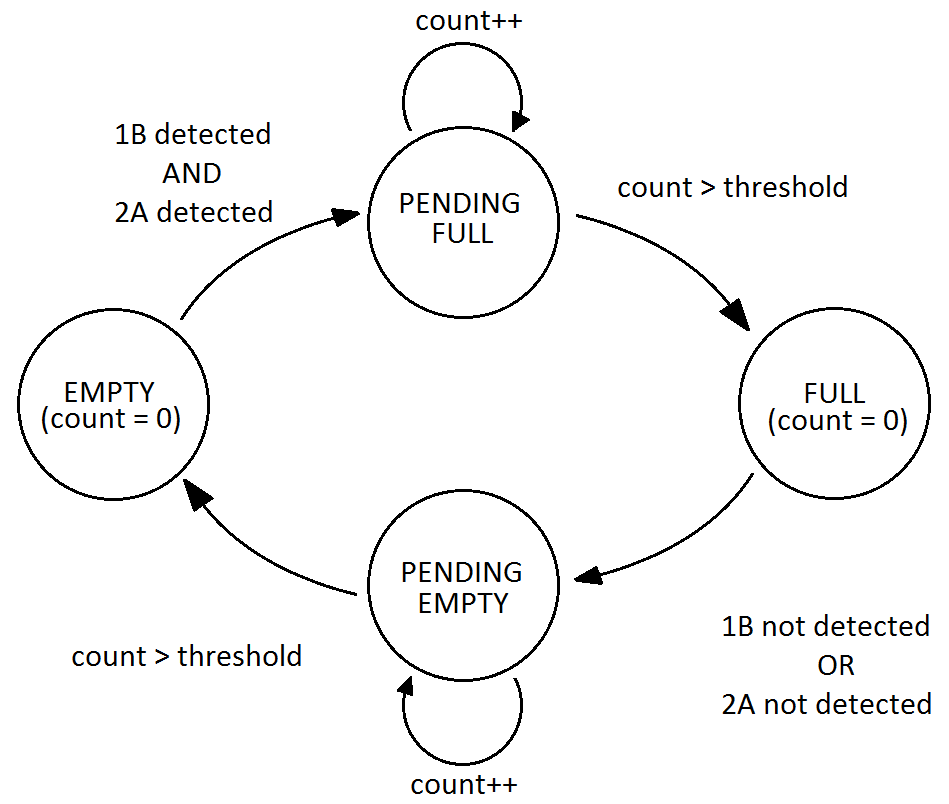
\includegraphics[width=2.5in]{FSM.png}
	\caption{Finite state machine for vehicle detection}
	\label{fig_fsm}
\end{figure}

A change in the two \texttt{proximity} bits that correspond to a parking space triggers a transition from \texttt{empty} or \texttt{full} to one of the ``pending'' states. The FSM then uses a counter to determine when to transition from a ``pending'' state to \texttt{full} or \texttt{empty}. If the change persists until \texttt{count} reaches a \texttt{threshold} value, the state transitions; otherwise, it reverts to the state before the ``pending'' state. Using a counter and a threshold filter out high-frequency events (e.g., pedestrians walking through parking spaces) and preserves low-frequency information (the presence/absence of a vehicle in the parking space). In this sense, \texttt{CarSensor}'s FSM is functionally equivalent to a \textit{switch debouncer}.

Note that \texttt{count} increments at the rate at which the sensor module sends new \texttt{proximity} data, so \texttt{threshold} represents a time duration. In our prototype, the value of \texttt{threshold} is 5, corresponding to 10 seconds.
\subsection{Smartphone app client}
We elected to use Android Studio\footnote{\url{https://developer.android.com/studio/index.html}} to build the end user's interface with our \texttt{CarSensor} system. This decision was largely motivated by our familiarity with Android Studio and our unfamiliarity with developing iOS apps.

The app, shown in Figure~\ref{fig_app}, is a simple TCP client that communicates with the server on port 8000. When the user presses ``CONNECT...,'' the app sends a request to the server and the server replies with its estimate of the state of the parking space(s).

\begin{figure}[h]
	\centering
	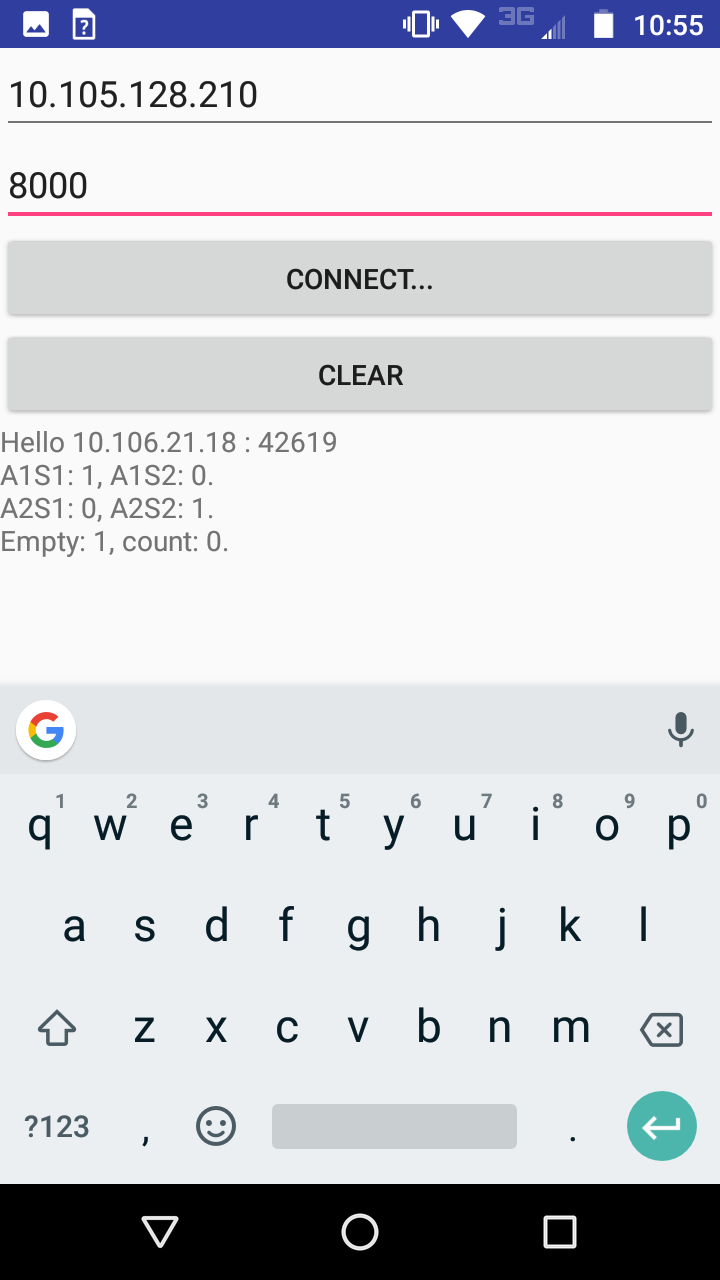
\includegraphics[width=2.0in]{app.png}
	\caption{Screenshot of the \texttt{CarSensor} Android app}
	\label{fig_app}
\end{figure}

To ease the development process, we provided a field for the user to enter the server's IP address, because it changed depending on whether we were working on campus or at home.

\section{Future Work}\label{sec_futurework}
While developing our prototype, we identified many avenues for improvement. Some of these ideas were not implemented due to limited time and/or technical prowess.
\subsection{Ease of use}
In the prototype, the user has to click ``connect'' every time he/she wants to see the newest information about parking spaces. An automatic notification feature would enhance the user experience. More fundamentally, the prototype app requires the user to know where each parking space is, which is unreasonable. A better app would integrate a maps-type feature with the existing notification system.
\subsection{Extensibility}
As alluded to in Section~\ref{sec_intro}, identifying each sensor module by IP address is a flawed approach for a couple reasons: first, IP address does not correlate with physical location, so the server cannot use IP addresses alone to reason about the state of each parking space; second, routers can only distribute a limited number of IP addresses. Clearly, a more considered approach is necessary. Programming each sensor module to transmit its ID along with its data also frees the server from having to know the IDs of all the sensor modules, thus making the system easier to expand.
\subsection{Robustness}
Recall that each sensor module transmits once every two seconds. This signal contains data (and could also contain an ID) but also functions like a heartbeat, in that its absence indicates the module's failure. The server simply needs to keep track of time since the last transmission from each sensor module. If ``too much'' time has elapsed since a particular module's last transmission, the server can advise a maintainer to check on that module.
\subsection{Power}
We offer two suggestions for improved power efficiency. We considered using solar power for our project but quickly decided against it, due to unnecessary complexity and the short time frame alloted for the project. Solar power is problematic because of fluctuating and unpredictable power output, so a batter and both charging and discharging circuits are also necessary. Nevertheless, solar power could be useful in a full-scale implementation of our system.

Our second recommendation is a low-power mode for the sensor modules. The ESP8266 draws up to 170 mA of current when transmitting. If the sensor module is running on a battery, a low-power mode with reduced transmission frequency (e.g., 0.05 Hz or even 0.005 Hz instead of 0.5 Hz) would extend battery life.
\subsection{Security}
We did not consider security risks when designing this prototype. There are two primary attack vectors: attacking the server through the app's port (port 8000) or through the sensor modules' port (port 8080). Neither of these requires authentication in our prototype, so they are security risks. A third (albeit more difficult) attack vector is through the sensor module itself: since the ATmega328P can be reprogrammed, it can be hacked. Countermeasures that achieve immunity to hacking without sacrificing reprogrammability warrant further investigation.
\section{Conclusion}\label{sec_conc}
We presented \texttt{CarSensor}, an IoT-inspired system for notifying drivers of the occupancy statuses of nearby parking spaces. The system is highly modular and consists of a physical layer and a network layer. We built a prototype using widely available open-source development tools, including the Arduino UNO, \texttt{Node.js}\textsuperscript{\textregistered}, and Android Studio. Our prototype demonstrated \texttt{CarSensor}'s viability and also illuminated a number of areas for improvement that are relevant to most cyberphysical systems.

\section*{References}
\begin{enumerate}
\item SparkFun ESP8266 AT Arduino Library. \url{https://github.com/sparkfun/SparkFun_ESP8266_AT_Arduino_Library}
\item \texttt{Node.js} main page. \url{https://nodejs.org/en/}
\item \texttt{Node.js} \texttt{net} API documentation. \url{https://nodejs.org/api/net.html\#net_net}
\item Android Studio main page. \url{https://developer.android.com/studio/index.html}

\end{enumerate}

\end{document}